\documentclass[journal,12pt,twocolumn]{IEEEtran}

\usepackage{setspace}
\usepackage{gensymb}
\singlespacing
\usepackage[cmex10]{amsmath}

\usepackage{amsthm}

\usepackage{mathrsfs}
\usepackage{txfonts}
\usepackage{stfloats}
\usepackage{bm}
\usepackage{cite}
\usepackage{cases}
\usepackage{subfig}

\usepackage{longtable}
\usepackage{multirow}

\usepackage{enumitem}
\usepackage{mathtools}
\usepackage{steinmetz}
\usepackage{tikz}
\usepackage{circuitikz}
\usepackage{verbatim}
\usepackage{tfrupee}
\usepackage[breaklinks=true]{hyperref}
\usepackage{graphicx}
\usepackage{tkz-euclide}

\usetikzlibrary{calc,math}
\usepackage{listings}
    \usepackage{color}                                            %%
    \usepackage{array}                                            %%
    \usepackage{longtable}                                        %%
    \usepackage{calc}                                             %%
    \usepackage{multirow}                                         %%
    \usepackage{hhline}                                           %%
    \usepackage{ifthen}                                           %%
    \usepackage{lscape}     
\usepackage{multicol}
\usepackage{chngcntr}

\DeclareMathOperator*{\Res}{Res}

\renewcommand\thesection{\arabic{section}}
\renewcommand\thesubsection{\thesection.\arabic{subsection}}
\renewcommand\thesubsubsection{\thesubsection.\arabic{subsubsection}}

\renewcommand\thesectiondis{\arabic{section}}
\renewcommand\thesubsectiondis{\thesectiondis.\arabic{subsection}}
\renewcommand\thesubsubsectiondis{\thesubsectiondis.\arabic{subsubsection}}


\hyphenation{op-tical net-works semi-conduc-tor}
\def\inputGnumericTable{}                                 %%

\lstset{
%language=C,
frame=single, 
breaklines=true,
columns=fullflexible
}
\begin{document}

\newcommand{\BEQA}{\begin{eqnarray}}
\newcommand{\EEQA}{\end{eqnarray}}
\newcommand{\define}{\stackrel{\triangle}{=}}
\bibliographystyle{IEEEtran}
\raggedbottom
\setlength{\parindent}{0pt}
\providecommand{\mbf}{\mathbf}
\providecommand{\pr}[1]{\ensuremath{\Pr\left(#1\right)}}
\providecommand{\qfunc}[1]{\ensuremath{Q\left(#1\right)}}
\providecommand{\sbrak}[1]{\ensuremath{{}\left[#1\right]}}
\providecommand{\lsbrak}[1]{\ensuremath{{}\left[#1\right.}}
\providecommand{\rsbrak}[1]{\ensuremath{{}\left.#1\right]}}
\providecommand{\brak}[1]{\ensuremath{\left(#1\right)}}
\providecommand{\lbrak}[1]{\ensuremath{\left(#1\right.}}
\providecommand{\rbrak}[1]{\ensuremath{\left.#1\right)}}
\providecommand{\cbrak}[1]{\ensuremath{\left\{#1\right\}}}
\providecommand{\lcbrak}[1]{\ensuremath{\left\{#1\right.}}
\providecommand{\rcbrak}[1]{\ensuremath{\left.#1\right\}}}
\theoremstyle{remark}
\newtheorem{rem}{Remark}
\newcommand{\sgn}{\mathop{\mathrm{sgn}}}
\providecommand{\abs}[1]{\vert#1\vert}
\providecommand{\res}[1]{\Res\displaylimits_{#1}} 
\providecommand{\norm}[1]{\lVert#1\rVert}
%\providecommand{\norm}[1]{\lVert#1\rVert}
\providecommand{\mtx}[1]{\mathbf{#1}}
\providecommand{\mean}[1]{E[ #1 ]}
\providecommand{\fourier}{\overset{\mathcal{F}}{ \rightleftharpoons}}
%\providecommand{\hilbert}{\overset{\mathcal{H}}{ \rightleftharpoons}}
\providecommand{\system}{\overset{\mathcal{H}}{ \longleftrightarrow}}
	%\newcommand{\solution}[2]{\textbf{Solution:}{#1}}
\newcommand{\solution}{\noindent \textbf{Solution: }}
\newcommand{\cosec}{\,\text{cosec}\,}
\providecommand{\dec}[2]{\ensuremath{\overset{#1}{\underset{#2}{\gtrless}}}}
\newcommand{\myvec}[1]{\ensuremath{\begin{pmatrix}#1\end{pmatrix}}}
\newcommand{\mydet}[1]{\ensuremath{\begin{vmatrix}#1\end{vmatrix}}}
\numberwithin{equation}{subsection}
\makeatletter
\@addtoreset{figure}{problem}
\makeatother
\let\StandardTheFigure\thefigure
\let\vec\mathbf
\renewcommand{\thefigure}{\theproblem}
\def\putbox#1#2#3{\makebox[0in][l]{\makebox[#1][l]{}\raisebox{\baselineskip}[0in][0in]{\raisebox{#2}[0in][0in]{#3}}}}
     \def\rightbox#1{\makebox[0in][r]{#1}}
     \def\centbox#1{\makebox[0in]{#1}}
     \def\topbox#1{\raisebox{-\baselineskip}[0in][0in]{#1}}
     \def\midbox#1{\raisebox{-0.5\baselineskip}[0in][0in]{#1}}
\vspace{3cm}
\title{AI 1103 - Assignment 4}
\author{T. Rohan \\ CS20BTECH11064}
\maketitle
\newpage
\bigskip
\renewcommand{\thefigure}{\theenumi}
\renewcommand{\thetable}{\theenumi}
Download all python codes from 
\begin{lstlisting}
https://github.com/rohanthota/Assignment_4/codes/Assignment_4.py
\end{lstlisting}
%
and latex codes from
%
\begin{lstlisting}
https://github.com/rohanthota/Assignment_4/Assignment 4.tex
\end{lstlisting}
\section*{\emph{Question}}
Let Z be the vertical coordinate, between -1 and 1, of a point chosen uniformly at random on the
\begin{math}
\text{surface of a unit sphere in }R^3.\text{ Then,} \pr{\frac{-1}{2} \leq Z \leq \frac{1}{2}}
\end{math}
is

\section*{\emph{Solution}}
The probabilities of various conditions, directly 
\\depend on the surface areas'.

\begin{math}
\text{Total surface area A} = 4\pi r^2 = 4\pi\brak{1^2} = 4\pi
\\\text{Here, we define random variable }X \in  \cbrak{0, 1}
\end{math}

\begin{math}
\text{Where,}
\\X = 0 \text{ when a point with } {\frac{-1}{2} \leq Z \leq \frac{1}{2}} \text{ is picked.}
\\X = 1 \text{ for all the other cases.}
\end{math}

\begin{align}
    \pr{X=0} &= \frac{\text{Area with }\frac{-1}{2} \leq Z \leq \frac{1}{2}}{\text{Total surface area}}
\end{align}
\begin{align}
\text{Considering area }A^\prime \text{ with } \frac{-1}{2} \leq Z \leq \frac{1}{2}
\end{align}
\\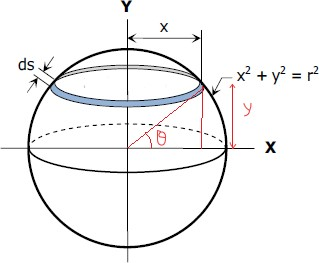
\includegraphics[width=65mm, height=50mm]{Surface area of sph diag}

\begin{align}
\text{Here x} &= r\cos{\theta}
\\\text{y} &=r\sin{\theta}
\\r^2 &= x^2 + y^2
\\ds &= rd\theta.
\end{align}
\begin{align}
    \text{Area of strip dA} &= 2\pi x\times ds
    = 2\pi  r\cos{\theta} \times rd\theta.
\end{align}
\begin{align}
    \text{For y} &=\frac{-1}{2}, \text{ }\theta = \frac{-\pi}{6}.
    \\\text{For y} &=\frac{1}{2}, \text{ }\theta = \frac{\pi}{6} 
\end{align}
\begin{align}
    A^\prime &= \int_{y = \frac{-1}{2}}^{y = \frac{1}{2}} dA = \int_{\frac{-\pi}{6}}^{\frac{\pi}{6}} 2\pi r^2 \cos{\theta} d\theta
    \\A^\prime &= 2\pi \brak{1}^2 \int_{\frac{-\pi}{6}}^{\frac{\pi}{6}} \cos{\theta} d\theta
    \\A^\prime &= 2\pi \sbrak{\sin{\theta}}_\frac{-\pi}{6}^\frac{\pi}{6} = 2\pi \sbrak{\frac{1}{2} - \frac{-1}{2}}
    \\\therefore A^\prime &= 2\pi
\end{align}
\begin{align}
    \therefore \pr{X = 0} &= \frac{A^\prime}{A} = \frac{2\pi}{4\pi} = \frac{1}{2}
\end{align}
\end{document}